\documentclass[]{article}
\usepackage{amsmath}\usepackage{amsfonts}
\usepackage[margin=1in,footskip=0.25in]{geometry}
\usepackage{mathtools}
\usepackage{hyperref}
\hypersetup{
    colorlinks=true,
    linkcolor=blue,
    filecolor=magenta,
    urlcolor=cyan,
}
\usepackage[final]{graphicx}
\usepackage{listings}
\usepackage{courier}
\lstset{basicstyle=\footnotesize\ttfamily,breaklines=true}
\newcommand{\indep}{\perp \!\!\! \perp}
% \usepackage{wrapfig}
\graphicspath{{.}}
% \usepackage{fancyvrb}

%%
%% Julia definition (c) 2014 Jubobs
%%
\usepackage[T1]{fontenc}
\usepackage{beramono}
\usepackage[usenames,dvipsnames]{xcolor}
\lstdefinelanguage{Julia}%
  {morekeywords={abstract,break,case,catch,const,continue,do,else,elseif,%
      end,export,false,for,function,immutable,import,importall,if,in,%
      macro,module,otherwise,quote,return,switch,true,try,type,typealias,%
      using,while},%
   sensitive=true,%
   alsoother={$},%
   morecomment=[l]\#,%
   morecomment=[n]{\#=}{=\#},%
   morestring=[s]{"}{"},%
   morestring=[m]{'}{'},%
}[keywords,comments,strings]%

\lstset{%
    language         = Julia,
    basicstyle       = \ttfamily,
    keywordstyle     = \bfseries\color{blue},
    stringstyle      = \color{magenta},
    commentstyle     = \color{ForestGreen},
    showstringspaces = false,
}
\begin{document}
\begin{center}
    Name: Hongda Li
    \\
    AMATH 585 HW4 2022 WINTER
\end{center}
\section*{Problem 1}
    Consider the boundary value problem: 
    $$
        \begin{cases}
            -\frac{d}{dx}\left(
                (1 + x^2)\frac{du}{dx}
            \right) = f(x) & \forall x \in [0, 1] 
            \\
            u(0) = u(1) = 0 & 
        \end{cases}
    $$
    \subsection*{(a)}
        \hspace{1.1em}
        \textbf{Objective}: Derive the Matrix equation that we will need to solve the problem, using Galerkin Finite Element Method, With continuous piecewise linear basis functions. For genericity when coding it into the computer, I make no assumptions about the meshgrid, or the actual implementations of integral approximations. 
        \par
        Introduce $\mathcal{L}[\cdot]:= \partial_x[r(x)\partial[\cdot]]$ as a differential operator; $\mathcal{S}$ denoing the basis for all the linear piecewise continous functions on $[0, 1]$ satisfying the boundary conditions, to derive, consider the weak form: 
        \begin{align*}\tag{1.a.1}\label{eqn:1.a.1}
            \langle \mathcal{L}[u], \varphi\rangle 
            &\equiv 
            -\int_{0}^1
            (\partial_x[r(x)\partial_x[u(x)]])\varphi(x)dx 
            = 
            \int_{0}^{1} f(x)\varphi(x)dx \equiv \langle f,\varphi\rangle
            \\
            &= 
            -\int_{0}^{1} 
                \varphi(x)
            d(r(x)u'(x))
            \\
            &= 
            -\left.\varphi(x)(r(x)u'(x))\right|_0^1
            +
            \int_{0}^{1} 
                r(x)u'(x)\varphi'(x)
            dx
            \\
            &= 
            -\varphi(1)r(1)\partial_x[u](1) + \varphi(0)r(0)\partial_x[u](0) + 
            \int_{0}^{1} 
                r(x)u'(x)\varphi'(x)
            dx
            = \langle f, \varphi\rangle
        \end{align*}
        Where, $\varphi(x)$ is some basis function in $\mathcal{S}$, in our case, let's say $\mathcal{S}$ is finite and has $n - 1$ elements (Because it's constructed on an discretized grid points: $[x_0, x_1, \cdots, x_n]$), and let $\varphi_i(x)$ is a basis function index by $i$ where $1\le i \le n -1$, then we have: 
        \begin{align*}\tag{1.a.2}\label{eqn:1.a.2}
            \varphi_i(x) &= 
            \begin{cases}
                \frac{x - x_{i - 1}}{x_i - x_{i - 1}} & x\in [x_{i - 1}, x_i)
                \\
                \frac{x_{i + 1} - x}{x_{i + 1} - x_{i}} & x\in [x_{i}, x_{i + 1}]
                \\
                0 & \text{else}
            \end{cases}
            \\
            \varphi_i'(x) &= \begin{cases}
                \frac{1}{x_{i} - x_{i - 1}} & x \in [x_{i - 1}, x_i)
                \\
                \frac{-1}{x_{i + 1} - x_{i}} & x \in (x_{i}, x_{i + 1}]
                \\
                \left[
                    \frac{-1}{x_{i + 1} - x_i}, \frac{1}{x_i - x_{i - 1}}
                \right]
                & x = x_i
                \\
                0 & \text{else}
            \end{cases}
        \end{align*}
        The objective of the finite elements method is to represents the solution, $u(x)$ as a linear combinations of the basis function $\varphi_j(x)$. Suppose that $\hat{u} = \sum_{j = 1}^{n - 1}c_j \varphi_j(x)$ and it's taking the dot product with another function $\varphi_i \in \mathcal{S}$ from the trial space, then reconsidering \hyperref[eqn:1.a.1]{(1.a.1)} the weak form and convert it to sysrem of linear equations: 
        \begin{align*}\tag{1.a.3}\label{eqn:1.a.3}
            &\hspace{1.1em} 
            -\varphi_i(1)r(1)\partial_x[u](1) + \varphi_i(0)r(0)\partial_x[u](0)
            + 
            \int_{0}^{1} 
                r(x)\partial_x[u(x)]\varphi_i'(x)
            dx
            \\
            &= 
            - \varphi_i(1)r(1)
            \sum_{j = 1}^{n - 1}
                c_j\varphi'_j(1)
            +
            \varphi_i(0)r(0)
            \sum_{j = 1}^{n - 1}
                c_j\varphi'_j(0)
            +
            \int_{0}^{1} 
                r(x)
                \sum_{j = 1}^{n - 1}c_j\varphi_j'(x)
                \varphi_i'(x)
            dx \tag{1.a.3.1}
            \\
            &= 0 + \sum_{j = 1}^{n - 1}
                \int_{0}^{1} 
                    r(x)c_j\varphi_j'(x)\varphi_i'(x)
                dx
        \end{align*}
        Going from (1.a.3.1) to the next line, we use the fact that for all basis function $\varphi_j(0) = 0 = \varphi_j(1), j=1,\cdots, n - 1$ by how the basis functions are defined. Take note that the above expression is true for all $\varphi_i$ where $1\le i \le n - 1$. 
        \par
        Above results will be true for all $\varphi_j\in \mathcal{S}$, from there we figure out the element of Differential Operator $A_{i, j}$, giving us: 
        \begin{align*}\tag{1.a.4}\label{eqn:1.a.4}
            A_{i, j}& = \int_{0}^{1} 
                r(x)\varphi_i'(x)\varphi_j'(x)
            dx
            \\
            &= 
            \int_{0}^{1} 
                (1 + x^2)\varphi_j'(x)\varphi_i'(x)
            dx
            \\
            &= \begin{cases}
                \int_{0}^{1} 
                    (1 + x^2)\varphi_j'(x)\varphi_i'(x)
                dx & |i - j| \le 1
                \\
                0 & \text{else }
            \end{cases}
        \end{align*}
        Take note that $\varphi_j'(x)$ is non zero on the domain $[x_{i - 1}, x_{i + 1}]$, which gives the tridiagonal structor of $A$, in addition, the expression remains the same if we swapped $i, j$, which means that the matrix $A$ is symmetric too. It's symmetric, and therefore we can decribe the elements on the diagonal and the sub-diagonal instead: 
        \begin{align*}\tag{1.a.5}\label{eqn:1.a.5}
            \forall\; 1 \le i \le n - 1 \; :
            A_{i, i} &= 
            \int_{0}^{1} 
                r(x)\varphi_i'(x)\varphi_i'(x)
            dx
            \\
            &= 
            \int_{x_{i - 1}}^{x_i} 
                r(x)\varphi_i'(x)^2
            dx +
            \int_{x_{i}}^{x_{i + 1}} 
                r(x)\varphi_i'(x)^2
            dx
            \\
            &= 
            \frac{1}{(x_{i} - x_{i - 1})^2}
            \int_{x_{i - 1}}^{x_i} r(x)dx
            + 
            \frac{1}{(x_{i + 1} - x_i)^2}\int_{x_{i}}^{x_{i + 1}} 
                r(x)
            dx
        \end{align*}
        Computing the Sub diagonals of Matrix $A$. 
        \begin{align*}\tag{1.a.6}\label{eqn:1.a.6}
            \forall\; 2 \le i \le n - 1 \; :
            A_{i - 1, i} = A_{i, i - 1} 
            &= 
            \int_{0}^{1} 
                r(x)\varphi_i'(x)\varphi_{i- 1}(x)
            dx
            \\
            &= 
                \int_{x_{i - 1 }}^{x_i} 
                    r(x)\varphi_i'(x)\varphi_{i - 1}'(x)
                dx
            \\
            &= 
            \int_{x{i}}^{x_{i - 1}} 
                r(x)
                \left(
                    \frac{1}{x_i - x_{i - 1}}
                \right)
                \left(
                    \frac{-1}{x_i - x_{i - 1}}
                \right)
            dx
            \\
            &= 
            \frac{-1}{(x_i - x_{i - 1})^2}
            \int_{x_{i - 1}}^{x_i} 
                r(x)
            dx
        \end{align*}
        For the RHS vector $\mathbf{f}$, we are deriving it from the weak form from \hyperref[eqn:1.a.1]{(1.a.1)}: 
        \begin{align*}\tag{1.a.7}\label{eqn:1.a.7}
            \forall\; 1 \le i \le n - 1\;: 
            \langle f(x), \varphi_i(x)\rangle
            &= 
            \int_{0}^{1} 
                f(x)\varphi_i(x)
            dx
            \\
            &= \int_{x_{i - 1}}^{x_i} 
                f(x)\varphi_i(x)
            dx + 
            \int_{x_i}^{x_{i + 1}} 
                f(x)\varphi_i(x)
            dx
            \\
            &= 
            \int_{x_{i - 1}}^{x_i} 
                \frac{f(x)(x - x_{i - 1})}{x_i - x_{i - 1}}
            dx - 
            \int_{x_i}^{x_{i + 1}}
                \frac{f(x)(x - x_{i + 1})}{x_{i + 1} - x_i}
            dx
            \\
        \end{align*}
        For our problem we have the choice to evaluate $r(x)$ either integrate by hand, or we can do it with Trapzoidal rules. When implemented on the computer, I implemented for both options. 
        \par
        $A$ is figured out in \hyperref[eqn:1.a.5]{(1.a.5)} ,\hyperref[eqn:1.a.5]{(1.a.6)} and $\mathbf{f}$ is figured out in \hyperref[eqn:1.a.7]{(1.a.7)}. 
    \subsection*{(b)}
        For Julia implementation refers to \hyperref[THECODE]{(the code)}
    \subsection*{(c)}
        The accuracy for the finite element method is $\mathcal{O}(h^2)$, and it's not changing wrt to the Qaussian Quadrature used to evaluate the integrals, but that does has an impact on the accuracy, but not the order of accuracy. 
        \begin{center}
            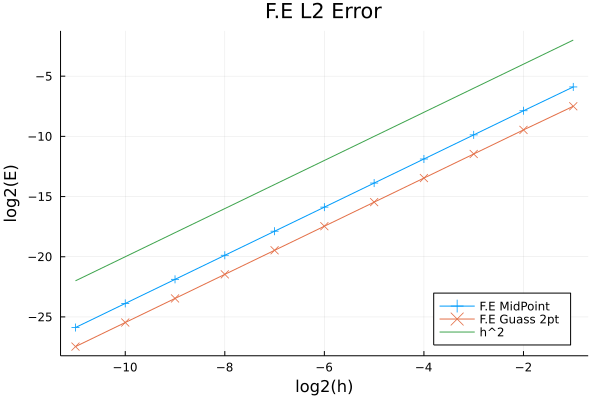
\includegraphics[width=10cm]{problem1C.png}
        \end{center}
        Grid points are evenly discretized and the grid width follows the sequence: $1/2, 1/4, ..., 1/2^{11}$. The error is measured in L2 norm. The function $\log_2(h^2)$ is plotted as an reference. 

    \subsection*{(d)}
        An grid point given by the function: $x_i = 1/(m + 1)^2, i = 0, \cdots, m + 1$, and we used $\max_{1\le i \le n}(x_i - x_{i - 1})$ on the x-axis, and the error is measured on the inf norm. 
        \begin{center}
            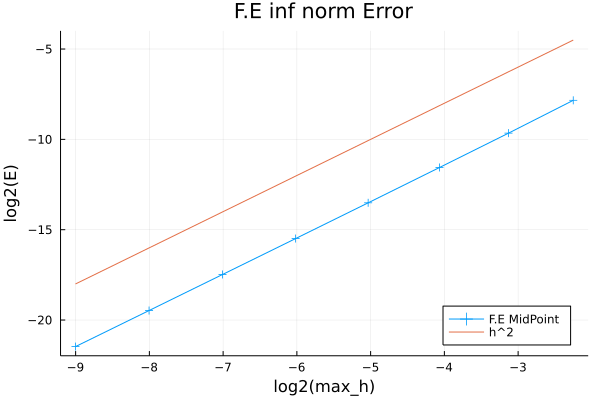
\includegraphics[width=10cm]{problem1D.png}
        \end{center}
        The function $\log_2(h^2)$ is plotted as an reference. The error is $\mathcal{O}(h^2)$.

    \subsection*{(e)}
        \hspace{1.1em}
        Here, we are interesting in solving the same steady state BVP problem, but with the boundary conditions: $u(0) = a, u(1) = b$. 
        \par
        We will have to use a new set of basis function and the Trial Space $\mathcal{S}$, because the previous basis deesn't contain functions to model the boundary conditions. To satisfy it, consider 2 extra basis function $\varphi_0(x), \varphi_{n}(x)$ where we can add to the set $\mathcal{S}$: 
        \begin{align*}\tag{1.e.1}\label{eqn:1.e.1}
            \varphi_0(x) &= 
            \begin{cases}
                \frac{x_1 - x}{x_1 - x_0}
                & 
                x \in [x_0, x_1]
                \\
                0 & \text{else}
            \end{cases}
            \implies 
            \varphi_0(x_0) = 1
            \\
            \varphi_{n}(x) &= 
            \begin{cases}
                \frac{x - x_{n - 1}}{x_n - x_{n - 1}}
                & 
                x\in [x_{n - 1}, x_n]
                \\
                0 & \text{else}
            \end{cases}
            \implies 
            \varphi_n(x_n) = 1
            \\
            \varphi_0'(x) &= \begin{cases}
                \frac{-1}{x_1 - x_0} & x\in [x_0, x_1]
                \\
                0 & \text{else}
            \end{cases}
            \implies \varphi_0'(x_0) = \frac{-1}{x_1 - x_0}
            \\
            \varphi_n'(x) &= 
            \begin{cases}
                \frac{1}{x_n - x_{n - 1}} & x\in [x_{n - 1}, x_n]
                \\
                0 & \text{else}
            \end{cases}
            \implies \varphi_n'(x_n) = \frac{1}{x_n - x_{n - 1}}
        \end{align*}
        \par
        As a consequence, we reconsider the form our solution $\hat{u}$ takes using the new basis of functions.
        \begin{align*}\tag{1.e.2}\label{eqn:1.e.2}
            \hat{u}(x) &= 
            a\varphi_0(x) + \sum_{j = 1}^{n - 1}c_j\varphi_j(x) + b\varphi_n(x)
        \end{align*}
        Take note that $\hat{u}(x)$ already satisfies the boundary conditions and $c\in \mathbb{R}^{n - 1}$. Now, we may reconsider the weak form derived from \hyperref[eqn:1.a.1]{(1.a.1)} by substituting our new $\hat{u}(x)$: 
        \begin{align*}\tag{1.e.3}\label{eqn:1.e.3}
            -\left.\varphi(x)r(x)u'(x)\right|_0^1
            +
            \int_{0}^{1} 
                r(x)u'(x)\varphi'(x)
            dx
            &= \langle f, \varphi\rangle
            \\
            \underset{\text{Substitute: } \hat{u}}{\implies}
            \left.
            -\varphi(x)r(x)\hat{u}'(x)
            \right|_0^1
            + 
            \int_{0}^{1} 
                r(x)\left(
                        a\varphi_0'(x)
                        + 
                        \sum_{j = 1}^{n - 1} c_j\varphi_j(x)
                        + 
                        b\varphi_n'(x)
                    \right)
            dx
            &= 
            \langle f, \varphi\rangle
            \\ 
            =
            \left.
            -\varphi(x)r(x)\hat{u}'(x)
            \right|_0^1
            + 
            \int_{0}^{1} 
                r(x)a\varphi_0'(x)\varphi(x)dx
            dx
            + 
            \sum_{j = 1}^{n - 1}
                \int_{0}^{1} 
                    r(x)c_j\varphi_j'(x)\varphi(x)
                dx&\cdots
            \\
            + 
            \int_{0}^{1}r(x)\varphi_n'(x)\varphi'(x) dx
            &= 
            \langle f, \varphi\rangle
        \end{align*}
        Take note that there are only $n - 1$ unknowns to determine, therefore when imposing the weak form, we can use $\{\varphi_j\}_{j = 1}^{n - 1}$, giving us:
        \begin{align*}\tag{1.e.4}\label{eqn:1.e.4}
            \forall\; 1 \le i \le n - 1: \; \hspace{10em}& 
            \\
            \underbrace{\left.
            -\varphi_i(x)r(x)\hat{u}'(x)
            \right|_0^1}_{=0 \quad(1.e.4.1)}
            + 
            \int_{0}^{1} 
                r(x)a\varphi_0'(x)\varphi_i(x)
            dx
            + 
            \sum_{j = 1}^{n - 1}
                \int_{0}^{1} 
                    r(x)c_j\varphi_j'(x)\varphi_i(x)
                dx&\cdots
            \\
            + 
            \int_{0}^{1}r(x)\varphi_n'(x)\varphi_i'(x) dx
            &= \langle f, \phi_i\rangle
        \end{align*}
        (1.e.4.1): Because $\varphi_i(x) = 0\; \forall\; 1 \le i \le n - 1$, which is from \hyperref[eqn:1.a.2]{(1.a.2)}, next, oberve that, forall $2 \le i \le n - 1$, this expression will be exactly the same as results from \hyperref[eqn:1.a.3]{(1.a.3)} because $\varphi_0(x) = 0 \;\forall x \in [x_0, x_1]$, and $\varphi_{n}(x) = 0 \;\forall\; x\in [x_{n - 1}, x_n]$, which means that $\varphi_0(x)\varphi_i(x) = 0\; \forall\; 2 \le i \le n - 1$, similarly $\varphi_n(x)\varphi_i(x)\; \forall\; 2 \le i \le n - 1$, which results in $\int_{0}^{1} r(x)a\varphi_0'(x)\varphi_i(x)dx = 0$ and $\int_{0}^{1}r(x)\varphi_n'(x)\varphi_i'(x) dx = 0$. 
        \par
        The part where \hyperref[eqn:1.e.4]{(1.e.4)} is different from \hyperref[eqn:1.a.3]{(1.a.3)} is when $i = 1, n - 1$, reconsidering it gives: 
        \begin{align*}\tag{1.e.5}\label{eqn:1.e.5}
            &\text{when } i = 1 
            \\
            & a\int_{0}^{1} 
                r(x)\varphi_0'(x)\varphi_1'(x)
            dx = \int_{x_0}^{x_1} 
                r(x)\frac{-a}{x_1 - x_0}\frac{1}{x_1 - x_0}
            dx
            \\
            &= \frac{-a}{(x_1 - x_0)^2}\int_{x_0}^{x_1} r(x)dx
            \\
            &
            b\int_{0}^{1} 
                r(x)\varphi_n'(x)\varphi_1'(x)
            dx = 0
            \\
            \implies
            \langle f, \varphi_1\rangle
            &= 
            \frac{-a}{(x_1 - x_0)^2}\int_{x_0}^{x_1} 
                r(x)
            dx + 
            \sum_{j = 1}^{n-1}
            \int_{0}^{1} 
                r(x)c_j\varphi_j'(x)\varphi_1(x)
            dx
            \\
            & \text{similarly when }i = n - 1
            \\
            & 
            a\int_{0}^{1} 
                r(x)\varphi_0'(x)\varphi_1'(x)
            dx = 0
            \\
            &
            b\int_{0}^{1} 
                r(x)\varphi_n'(x)\varphi_{n - 1}'(x)
            dx 
            =
            b\int_{x_{n - 1}}^{x_n} 
                r(x)\frac{1}{x_n - x_{n - 1}}\frac{-1}{x_n - x_{n - 1}}
            dx
            \\
            & = 
            \frac{-b}{(x_n - x_{n - 1})^2}\int_{x_{n - 1}}^{x_n} 
                r(x)
            dx
            \\
            \implies
            \langle f, \varphi_{n - 1}\rangle
            &= 
            \frac{-b}{(x_n - x_{n - 1})^2}\int_{x_{n - 1}}^{x_n} 
                r(x)
            dx + 
            \sum_{j = 1}^{n - 1}
            \int_{0}^{1} 
                r(x)c_j\varphi'(x)\varphi_{n - 1}'(x)
            dx
        \end{align*}
        That is, only the first and the last row of $A\mathbf{c} = \mathbf{f}$ is modified when the boundary conditions changed from $u(1) = u(0) = 0$, and for B.C with $u(0) = a, u(1) = b$, we can change the RHS to $\tilde{\mathbf{f}}$, where $\tilde{\mathbf{f}}$ is just: 
        \begin{align*}\tag{1.e.6}\label{eqn:1.e.6}
            \tilde{\mathbf{f}} &= 
            \mathbf{f} + 
            \begin{bmatrix}
                \frac{a}{(x_1 - x_0)^2}\int_{x_0}^{x_1} 
                    r(x)
                dx
                \\
                0
                \\
                \vdots 
                \\
                0 
                \\
                \frac{b}{(x_n - x_{n - 1})^2}\int_{x_{n - 1}}^{x_n} 
                r(x)
                dx
            \end{bmatrix}
        \end{align*}
        Then the system $A\mathbf{c} = \tilde{\mathbf{f}}$ will solve B.C: $u(0) = a; u(1) = b$. 
        \subsection*{F.E Julia implementations}\label{THECODE}
            \begin{lstlisting}
function MidPointRuleSingleInterval(f::Function, a, b)
return (b - a)*f((a/2 + b/2)) end



function TrapzRuleSingleInterval(f::Function, a, b)
return (b - a)*(f(a)/2 + f(b)/2) end



function TwoPointsGaussQuadratureSingleInterval(f::Function, a, b)
    m = a/2 + b/2
    l = m - (1/sqrt(3))*(m - a)
    r = m + (1/sqrt(3))*(b - m)
return 0.5*(b - a)*(f(l) + f(r)) end


"""
    A specific steady state BVP finite element problem. 
    -(r(x)u'(x))' = f(x), x in [0, 1], u(0) = alpha, u(1) = beta
    Using:  
        - Any user defined mesh grid in 1D. 
        - Piecewiese Linear Basis function only. 

    * Field Explanations
        - 
"""
mutable struct FiniteElementProblem{T<:Number}
    r::Function         # heat conductivity
    alpha::T            # left boundary condition, dirichlet
    beta::T             # right boundary condition, dirichlet
    f::Function         # RHS function
    integral_rule:: Function
                        # an implementation of taking integral. 

    x_grids::AbstractVector{T}
                        # Number of grid inner grid points for the problem, 
                        # includes the boundary. 
    max_h::T            # Maximum meshgrid spacing. 

    A::AbstractMatrix{T}# Discrete Linear Operator for F.E. 
    rhs::Vector{T}                 # The rhs function INCLUDING the boundary conditions. 
    c::Vector{T}                   # Weights on Basis Functions. 

    """
        NOTE: Constructor limited the type of T = AbstractFloat. 
    """
    function FiniteElementProblem(
        r::Function, 
        f::Function, 
        alpha, 
        beta, 
        x_grids::AbstractVector,
        integral_rule::Function=MidPointRuleSingleInterval
    )
        this = new{AbstractFloat}()
        this.r = r
        this.f = f
        this.integral_rule = integral_rule
        this.alpha = alpha
        this.beta = beta
        @assert length(x_grids) >= 3 "Given Grid points must have more"*
        " than 3 elements but we have $(length(x_grids))"
        @assert ndims(x_grids) == 1 "The grid point has to be a 1D vector,"*
        " but we have: $(ndims(x_grids))"
        this.x_grids = copy(x_grids)
        this.max_h = maximum(x_grids[2:end] - x_grids[1:end - 1])
        
        @assert minimum(x_grids[2:end] - x_grids[1:end - 1]) > 0 "Meshgrid Error."
        
        MakeDiscreteOperator!(this)    
        MakeRHS!(this)

    return this end

end

"""
    Re-estrablish the discretized operator in the field 
    of the struct using the current parameters in the struct. 
"""
function MakeDiscreteOperator!(this::FiniteElementProblem)
    # make diagonals
    diagonal = Vector()
    subdiagonal = Vector()
    for (xl, xm, xr) in zip(
        this.x_grids[1:end - 2], 
        this.x_grids[2:end - 1],
        this.x_grids[3:end]
    )
        push!(
            diagonal, 
            this.integral_rule(this.r, xl, xm)/(xm - xl)^2 +
            this.integral_rule(this.r, xm, xr)/(xr - xm)^2
        )
    end

    # make sub-diagonals
    for (xl, xr) in zip(
        this.x_grids[2:end - 2], 
        this.x_grids[3:end - 1]
    )
        push!(
            subdiagonal, 
            -this.integral_rule(this.r, xl, xr)/(xr - xl)^2
        )

    end
    this.A = SymTridiagonal(diagonal, subdiagonal)
return end


"""
    establish the new RHS for the finite element equation using the 
    current parameters defined in the struct. 
"""
function MakeRHS!(this::FiniteElementProblem)
    rhsVec = Vector()
    func(x, z) = this.f(x)*(x - z)
    for (xl, xm, xr) in zip(
        this.x_grids[1:end - 2], 
        this.x_grids[2:end - 1],
        this.x_grids[3:end]
    )
        push!(
            rhsVec, 
            this.integral_rule((x) -> func(x, xl), xl, xm)/(xm - xl) - 
            this.integral_rule((x) -> func(x, xr), xm, xr)/(xr - xm)
        )

    end
    rhsVec[1] += (this.alpha/(this.x_grids[2] - this.x_grids[1])^2)*
        this.integral_rule(this.r,this.x_grids[1], this.x_grids[2])
    rhsVec[end] += (this.alpha/(this.x_grids[end] - this.x_grids[end - 1])^2)*
    this.integral_rule(this.r,this.x_grids[end - 1], this.x_grids[end])
    this.rhs = rhsVec
return end

"""
    Given a series of points to query the solution value at, 
    we solve this the system. 
"""
function Solve(this::FiniteElementProblem)
    if !isdefined(this, :c)
        this.c = this.A\this.rhs
    end
return copy(vcat(this.alpha, this.c, this.beta)) end



## Using this code to solve some problems in HW. 

using LinearAlgebra, Plots, Logging

function BasicTests()
    xgrid = LinRange(0, 1, 11)
    r(x) = (1 + x^2)
    alpha, beta = 0, 0
    delta = 0.1
    f(x) = 2*(3x^2 - x + 1)
    P = FiniteElementProblem(r, f, alpha, beta, xgrid, TwoPointsGaussQuadratureSingleInterval)
    fig = plot(xgrid, Solve(P), label="F.E Soln")
    plot!(fig, LinRange(0, 1, 1000), (x)-> x*(1 - x), label="u(x)") |> display
    
return P end

P = BasicTests();

"""
    Uniform Grid Point Error Plot
"""
function Problem1PartC()
    r(x) = (1 + x^2)
    alpha, beta = 0, 0
    f(x) = 2*(3x^2 - x + 1)
    u(x) = x*(1 - x)
    gridPoints = 1:11
    ErrorsMidPoint = Vector{AbstractFloat}()
    ErrorGauss = Vector{AbstractFloat}()
    GridSize = Vector{AbstractFloat}()
    for m in 2 .^(collect(gridPoints)) .+ 1
        xgrid = LinRange(0, 1, m) |> collect
        P = FiniteElementProblem(r, f, alpha, beta, xgrid)
        P2 = FiniteElementProblem(
            r, f, alpha, beta, xgrid, TwoPointsGaussQuadratureSingleInterval
        )
        solved = Solve(P)
        solved2 = Solve(P2)
        push!(GridSize, P.max_h)
        push!(ErrorsMidPoint, sqrt(P.max_h)*norm(solved - u.(xgrid)))
        push!(ErrorGauss, sqrt(P.max_h)*norm(solved2 - u.(xgrid)))
    end
    fig = plot(
        GridSize.|>log2, 
        ErrorsMidPoint.|>log2, 
        markershape=:+, 
        label="F.E MidPoint",
        legend=:bottomright, 
        xlabel="log2(h)",
        ylabel="log2(E)",
        title="F.E L2 Error"
    )
    plot!(
        GridSize .|> log2, 
        ErrorGauss .|> log2, 
        markershape=:x, 
        label="F.E Guass 2pt"
    )
    plot!(GridSize.|>log2, GridSize.^2 .|> log2, label="h^2")
    fig |> display
    savefig(fig, "problem1C.png")
return end

Problem1PartC()


"""
Non Uniform Grid Point Plots: 
"""
function ProblemPartD()
    # Prblem parameters: 
    r(x) = (1 + x^2)
    alpha, beta = 0, 0
    f(x) = 2*(3x^2 - x + 1)
    u(x) = x*(1 - x)
    gridSize = Vector{Float64}()
    Errors = Vector{Float64}()
    for m in 2 .^collect(3:10)
        xgrid = (((0:m + 1) |> collect)/(m + 1)).^2
        P = FiniteElementProblem(
            r, f, alpha, beta, xgrid
        )
        solved = Solve(P)
        push!(gridSize, P.max_h)
        push!(Errors, (solved - u.(xgrid))|>maximum)
    end
    fig = plot(
        gridSize.|>log2, 
        Errors.|>log2, 
        markershape=:+, 
        label="F.E MidPoint",
        legend=:bottomright, 
        xlabel="log2(max_h)",
        ylabel="log2(E)",
        title="F.E inf norm Error"
    )
    plot!(gridSize.|>log2, gridSize.^2 .|> log2, label="h^2")
    fig |> display
    savefig(fig, "problem1D.png")
return end

ProblemPartD()
            \end{lstlisting}

\section*{Problem 2}


\end{document}